\documentclass[11pt,oneside,a4paper]{article}
\usepackage{graphicx}
\usepackage{booktabs}
\usepackage{caption}
\usepackage{subcaption}
\usepackage{amsmath}
\usepackage{amsfonts}
\usepackage{amssymb}
\usepackage{lscape}
\usepackage{psfrag}
\usepackage[usenames]{color}
\usepackage{bbm}
\usepackage[update]{epstopdf}
\usepackage[bookmarks,pdfstartview=FitH,a4paper,pdfborder={0 0 0}]{hyperref}
\usepackage{verbatim}
\usepackage{listings}
\usepackage{textcomp}
\usepackage{fancyhdr}
\usepackage{multirow}
\pagestyle{fancy}
\usepackage{tikz}
\usepackage{course}
\usepackage{csvsimple}
\usepackage{float}

\renewcommand{\sectionmark}[1]{\markboth{#1}{#1}}
\renewcommand{\subsectionmark}[1]{\markright{#1}}

\fancyhf{}
\fancyhead[RO]{\nouppercase{\footnotesize\sc\leftmark\ \hrulefill\ \thepage}}
\fancyhead[RE]{\nouppercase{\footnotesize\sc\thepage\ \hrulefill\ }}
\renewcommand{\headrulewidth}{0pt}

\makeatletter
\def\cleardoublepage{\clearpage\if@twoside \ifodd\c@page\else%
	\hbox{}%
	\thispagestyle{empty}%
	\clearpage%
	\if@twocolumn\hbox{}\clearpage\fi\fi\fi}
\makeatother


\renewcommand{\topfraction}{0.9}  % max fraction of floats at top
\renewcommand{\bottomfraction}{0.8} % max fraction of floats at bottom
% Parameters for TEXT pages (not float pages):
\setcounter{topnumber}{2}
\setcounter{bottomnumber}{2}
\setcounter{totalnumber}{4}            % 2 may work better
\setcounter{dbltopnumber}{2}           % for 2-column pages
\renewcommand{\dbltopfraction}{0.9}    % fit big float above 2-col. text
\renewcommand{\textfraction}{0.07}     % allow minimal text w. figs
% Parameters for FLOAT pages (not text pages):
\renewcommand{\floatpagefraction}{0.7}  % require fuller float pages
% N.B.: floatpagefraction MUST be less than topfraction !!
\renewcommand{\dblfloatpagefraction}{0.7} % require fuller float pages

\sloppy

\widowpenalty=10000
\clubpenalty=10000

\edef\today{%\number\day\
	\ifcase\month\or
	January\or February\or March\or April\or May\or June\or July\or
	August\or September\or October\or November\or December\fi\ \number\year}
\title{\vspace*{40.0mm}
	\bf\sf Design of a structured product
	\vspace*{20.0mm} \\
	\vspace*{40.0mm}
	%\vspace{-20mm}\framebox{DRAFT VERSION}\vspace{20mm} \\
	% \Large\bf\sf Design of a structured product \vspace*{20.0mm}}
}
\author{\sf Tim Buchholz}
\date{\sf 21.10.20}

\begin{document}
	
	\begin{figure}
		\parbox[t]{125mm}{
			\vspace*{6mm}
			\scriptsize\sf           FACULTY OF ENGINEERING SCIENCE\\
			\scriptsize\sf\bfseries  Fundamentals of Financial Mathematics \\
			\scriptsize\sf           Home Assignment 2020-2021 \\
			\scriptsize\sf           Tim Buchholz}
		\parbox[t]{40mm}{
			\begin{flushright}
				
\includegraphics[height=15mm]{logo-eps-converted-to.pdf}
		\end{flushright}}
	\end{figure}
	
	\maketitle
	\thispagestyle{empty}
	\raggedbottom
	
	\cleardoublepage
	\pagenumbering{roman}
	\setcounter{tocdepth}{2}
	
	\tableofcontents
	
	\cleardoublepage
	\pagenumbering{arabic}
	
	\section{Introduction, Assumptions and relevant market data}
	In this assignment the design of two structured products for an underlying stock will be discussed. Namely the underlying stock is Advanced Micro Devices, Inc. , which is also known as AMD. AMD is an American multinational semiconductor company, which produces Computer processors and related technologies for business and consumer markets. 
	For many investors AMD is a really interesting company, as it is beside of Intel (Intel Corp. v. Advanced Micro Devices) the biggest producer for computer processors with even growing partial of the market. 
	Additionally the recent release of the new graphics processing units (GPUs) is very promising as these represent serious competition to Nvidia graphics cards, which dominated the market in the last years.
	
	Following structured products will be introduced:
	\begin{itemize}
		\item Product 1: Partially principal protected note
		\item Product 2: Airbag note
	\end{itemize}
	As underlying Finance instruments we will basically consider three different assets:
	\begin{itemize}
		\item the risk-free bank account with an fixed interest rate $r$
		\item the stock $ S $ (in this case AMD)
		\item Call and Put options on the stock S
	\end{itemize}
	As starting date $ t=0 $ Friday the 20st November is choosen.
	The maturity date of the products is Friday 21st January 2022.
	More precisely the structured product, which will be discussed later, are build on the data presented below, accessed at Friday 20st November at 4:45 pm (MEZ), which is one hour and a quarter after the market opening at that day. The stock price at this moment was $ S_0=85.35 \text{ USD} $. The data is shown in the tables at the end of this section. A small extract of the data is moreover shown in a associated screenshot in the appendix. As the tables already contain the full data, the screenshot only shows the stock price and the first few call options.  \\


	To get a fixed interest rate for the whole time period, the daily treasure yield rate of the US treasure bond at the starting date $ t=0 $ is picked, which we denote by $ r = 0.11 \% $.
	In the appendix also an associated table is shown, which is published at \cite{site_treasure}
    an official website of the United States Government.
   
	
	
	The reason of choice is that the base interest rate of the United States, the United States Fed Funds Rate, is given by a target range of $ 0-0.25 \% $. Moreover the Daily Treasury Yield Curve Rates are given for different time periods exactly. Since the time period of our products is around one year and two months the rate for an investment over one year is picked. As the investment is even longer than one year, that is a rather cautious estimate for the interest rate.
	
	
		\begin{table*}[!ht]
		\csvreader[%
		tabular={|c|c|c|c|c|c|c|},
		table head = \hline\textbf{{LastTradeDate}} & \textbf{Strike} & \textbf{LastPrice} & \textbf{Bid} & \textbf{Ask}  & \textbf{Volume} & \textbf{ImpliedVolatility}\\\hline,
		late after line= \\,
		late after last line=\\\hline %
		]{../data/yahoo_pc_stat_210122_table0_20112020_16:45:35}{LastTradeDate=\LastTradeDate,Strike=\Strike,LastPrice=\LastPrice,Bid=\Bid,Ask=\Ask,Volume=\Volume,ImpliedVolatility=\ImpliedVolatility}%
		{\LastTradeDate &\Strike & \LastPrice & \Bid & \Ask & \Volume & \ImpliedVolatility}
		\centering
		\caption{\label{table1}European Call Options AMD (data extracted from \cite{site_yahoofinance} at 20/11/2020 16:45:35)}
	\end{table*}
	\begin{table*}[!ht]
		\csvreader[%
		tabular={|c|c|c|c|c|c|c|c|},
		table head = \hline\textbf{{LastTradeDate}} & \textbf{Strike} & \textbf{LastPrice} & \textbf{Bid} & \textbf{Ask} & \textbf{Volume} & \textbf{ImpliedVolatility}\\\hline,
		late after line= \\,
		late after last line=\\\hline %
		]{../data/yahoo_pc_stat_210122_table1_20112020_16:45:35}{LastTradeDate=\LastTradeDate,Strike=\Strike,LastPrice=\LastPrice,Bid=\Bid,Ask=\Ask,Volume=\Volume,ImpliedVolatility=\ImpliedVolatility}%
		{\LastTradeDate &\Strike & \LastPrice & \Bid & \Ask & \Volume & \ImpliedVolatility}
		\centering
		\caption{\label{table2}European Put Options AMD (data extracted from \cite{site_yahoofinance} at 20/11/2020 16:45:35)}
	\end{table*}
	\newpage
	\section{Product 1: Partially principal protected note (PPPN)}
	\subsection{Descriptive part: What is a PPPN and why is it interesting?}
	A partially principal protected note (PPPN) is an investment option over an underlying stock, in our case AMD. Many people are initially skeptical when it comes to investing in stocks. The reason for this is that the opportunities come with risks. A PPPN is en investment option, where the risk is partially absorbed. Imagine for instant investing $850 \text{ USD}$ in a PPPN with fixed maturity date $ T $ over an underlying stock with initial stock price $ S_0 = 85 \text{ USD} $.
	\begin{figure}[H]
		\centering
		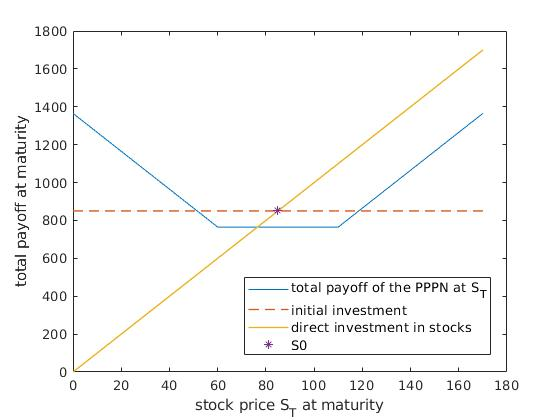
\includegraphics[width=0.8\linewidth]{payoff_PPPN.jpg}
		 \caption{payoff for an PPPN}
	\end{figure} 
	
	\subsection{Technical Part: How does a PPPN work?}
	\newpage
	\section{Product 2: Airbag note (AN)}
	\subsection{Descriptive part: What is a AN and why is it interesting?}
	\subsection{Technical Part: How does a AN work?}
	\cleardoublepage
	\section{Appendix}
	\subsection{Screenshot of the market data}
	\begin{figure}[H]
		\centering
		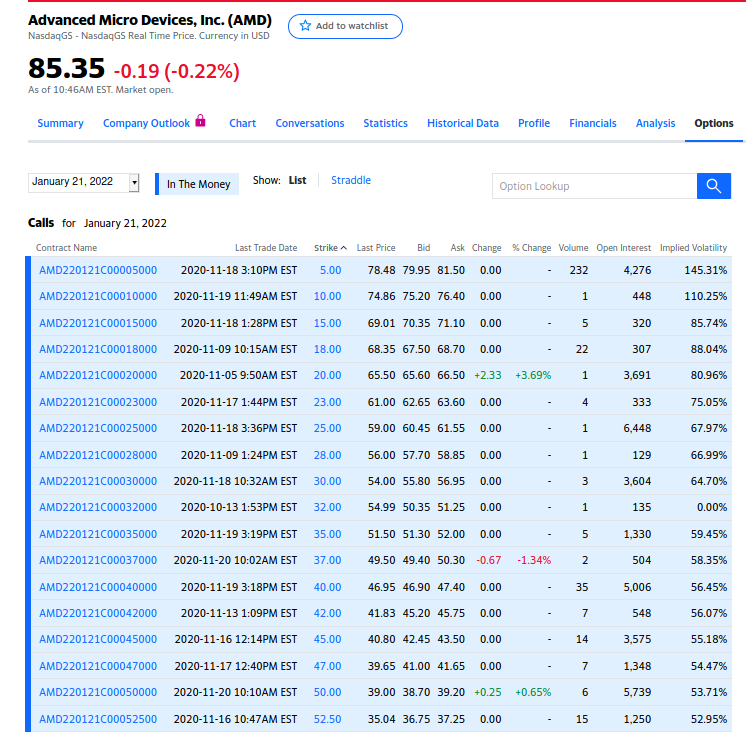
\includegraphics[width=\linewidth]{screenshot.png}
		\caption{\label{treasure}Small extract of the relevant market data from \cite{site_yahoofinance}} 
	\end{figure}
	\subsection{Daily Treasury Yield Curve Rates}
	\begin{figure}[H]
		\centering
		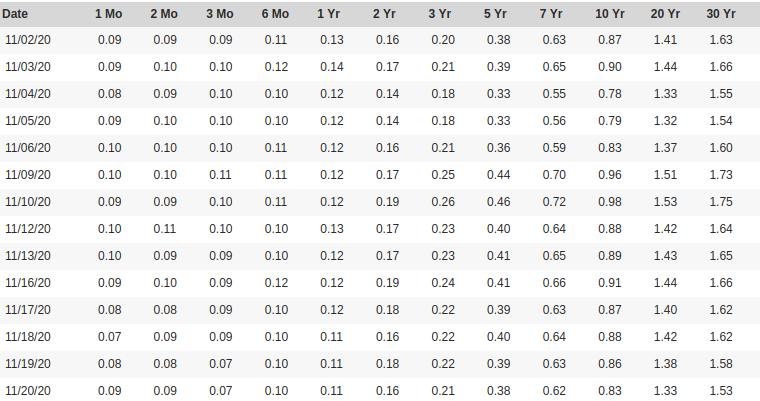
\includegraphics[width=0.8\linewidth]{treasure.png}
		\caption{\label{treasure}Daily Treasury Yield Curve Rates from \cite{site_treasure}} 
	\end{figure}
	\newpage
	\bibliographystyle{abbrv}
	\bibliography{References}
	
	 
\end{document}